\documentclass[../ClassicThesis.tex]{subfiles}
\begin{document}

%************************************************
\chapter{Joint Computation}\label{ch:joints}
%************************************************

% Use active Voice (we do….)
% Ein Gedanke pro Paragraph
% Terminologie anpassen über alle Arbeiten hinweg (was ist eine Plate für alle…)
% Jeder sollte eine kleine Related Work section haben
% Erklärungen zu warum dieser Algorithmus genutzt wurde und nicht ein anderer + limitations des gewählten Algorithmus
% Hübsche Bildchen zum anschaulichen Erklären!! (ebenfalls konsistent halten: gleich geformte labels etc.)

\section{Joint computation}
\textbf{TODO: buy green and orange (or at least two different colors) of acrylic for demo objects and pictures in the paper}
\paragraph{Overview Paragraph: what will be achieved, why is it necessary}
When an object consisting of multiple parts is lasercutted it needs to have connectors. Those can be elements like screws, nails and glue. Or the plates already come along with connectors. Those can be for example fingerjoints which, when well calibrated, do not need any external material to hold together. \\
Whenever possible we want to provide connections like that because a user needs less effort, when components work directly out of the lasercutter. This is why we provide three types of joints which are added to the determined plates.

\subsection{Volume based clipping}
Before joints can be added to the plates we have to prepare them. We cut the shapes back so that the joints do not overlap with the other plate.
\paragraph{prerequisite: plategraph intersection lines}
As seen before in the step [plateGraph] up to four intersectionlines will have been calculated.\\
Two of them lie both on one side of the plate and the other two belong to the second side. The two lines on one side build a rectangle when their ends are connected. We use those two rectangles to cut out of the plate what will get fingerjoints.\\
%\textbf{TODO: Insert image of the four lines, with the two rectangles marked.}\\
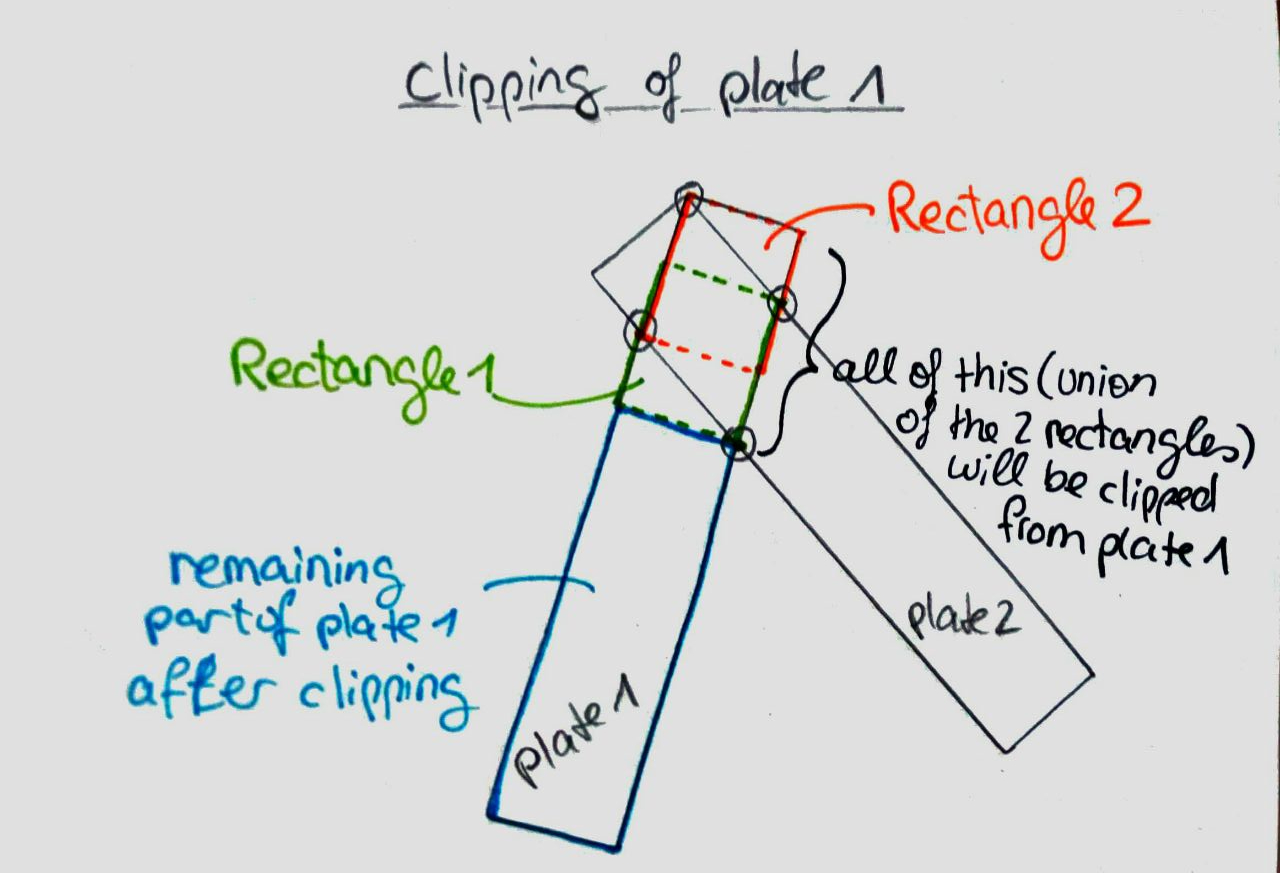
\includegraphics[width=\columnwidth]{Images/10-joints-clippingPlate.jpg}\\
There are cases when not all four lines are actually a plate intersection but only a plane intersection. \\
%\textbf{TODO: Image of plates which result in not 4 intersections.}\\
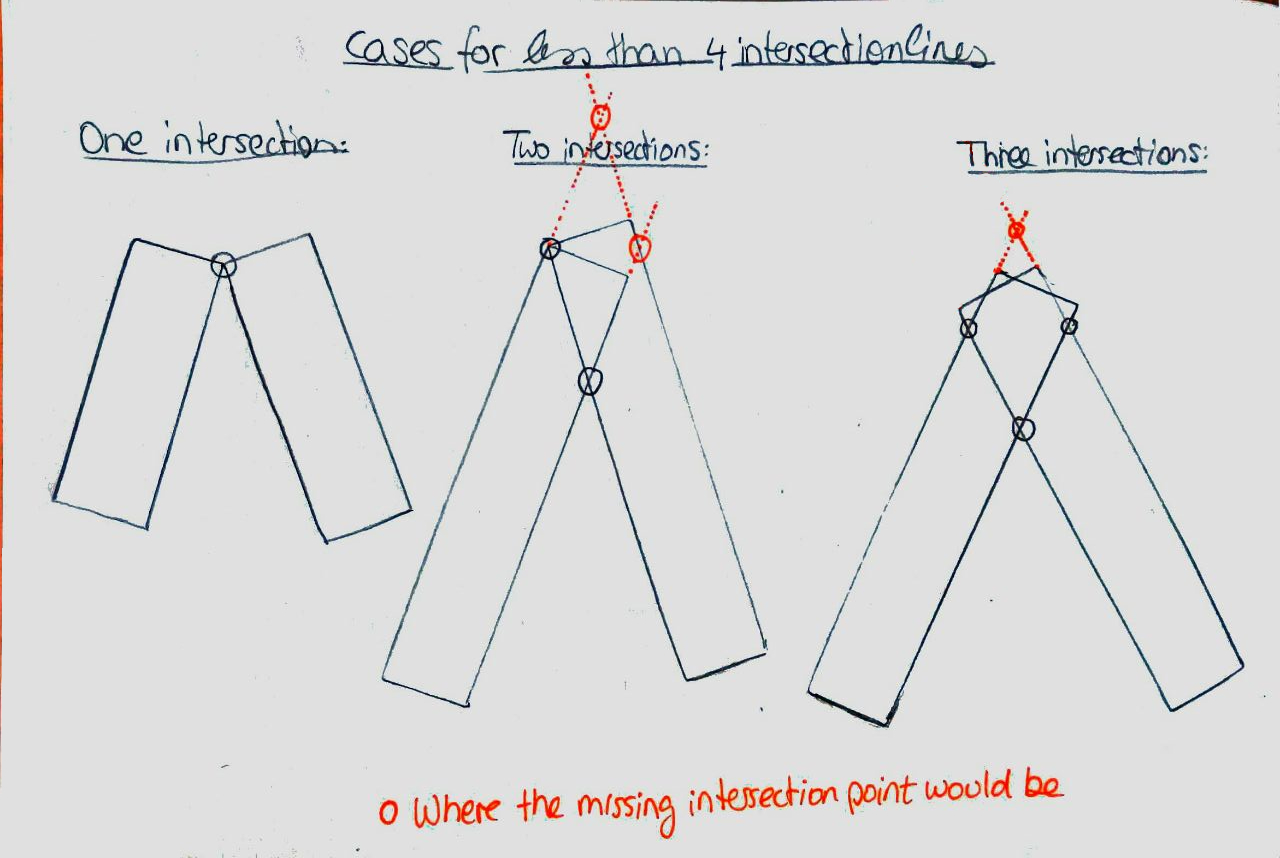
\includegraphics[width=\columnwidth]{Images/10-joints-casesOfLines.jpg}\\
In this case the infinitifly long plane intersection line will be clipped to match the length of the existing plate intersections. This yields two rectangles as well, which can then be used for clipping the shapes of the plates.



\section{building joints}
The general procedure of creating joints is achieved in three steps: First we calculate how many female and male joints fit onto the intersection. Then the retrieved joints are placed at the intersectionline and finally the shapes are merged to result in the original plate with joints.
\begin{enumerate}
    \item buildAlignedJointTemplates\\
        \paragraph{jointCount}
        We need to know how many joints we have to place onto the intersection. We call this 'jointCount' which describes the number of all joints to fit on the line including the male and female joints. Since all joint types have equal widths for female and male joints we divide the length of the line by the width of a joint.
        \paragraph{adjustJointWidth}
        But this calculation has to be rounded which means the number of joints just found might not fill the complete length of the line after all. Therefore we adjust the width so that the joints will be evenly spread without leaving space on either end of the line.
        Now that we know how the joints will look like and how many we need it is time to find out how to distribute them.\\
        We defined that when there is an even number of joints, the middle joint will be male and twice as thick as normally.\\
        %\textbf{TODO: provide image of the two cases: even and odd number}
        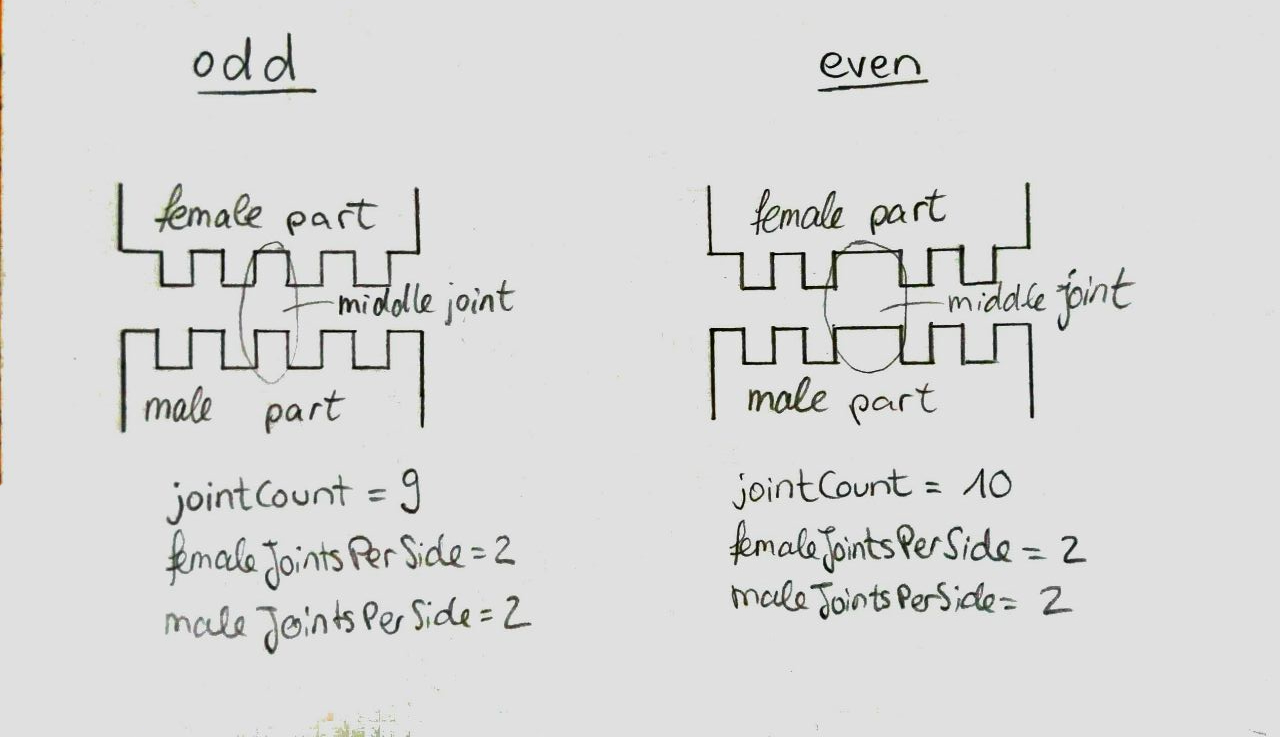
\includegraphics[width=\columnwidth]{Images/10-joints-evenOddJointCount.jpg}
        \paragraph{computeMaleJointsPerSide} %number only
        On both sides of the middle joint will be an equal number of male joints. How many depends on the jointCount. An even jointCount means 2 joints less and odd means one joint less on the sides because the middle joint will be created seperately. Since the jointCount specifies the number of all joints, male and female we have to divide by two to get the number of male joints only and then divide by two once more to achieve the seperation into the two sides.\\
        maleJointsPerSide = 
        \begin{cases} 
        (jointCount - 2) / 4, & jointCount $ \% 2 == 0 $ \\ 
        (jointCount - 1) / 4, & jointCount $ \% 2 == 1 $
        \end{cases}
            \paragraph{buildJointsForEven / Odd count}
            Finally, we can start placing the middle joint and distributing as many joints as just calculated on either side of it evenly with leaving enough space inbetween the joints for a female one to fit in.\\
            % \textbf{TODO: image of final spreaded joints, show that distance between them is the width.}
            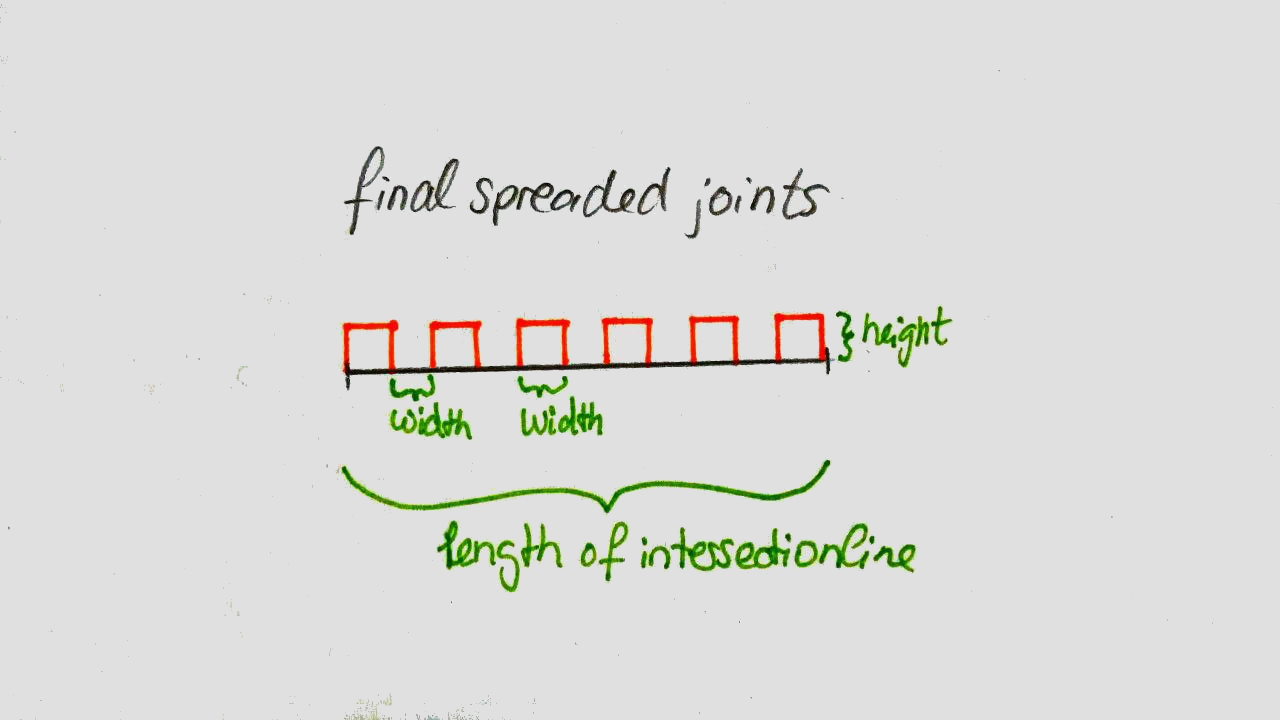
\includegraphics[width=\columnwidth]{Images/10-joints-spreadedJoints.jpg}
        \paragraph{computeFemaleJointsPerSide} %number only
        The computation for the number of female joints on one side of the middle joint is very similar to the previous computation for male joints. Only that the middle joints do not have to be subtracted.\\
        femaleJointsPerSide = 
        \begin{cases} 
        (jointCount) / 4, & jointCount $ \% 2 == 0 $ \\ 
        (jointCount + 1) / 4, & jointCount $ \% 2 == 1 $
        \end{cases}
            \paragraph{create Females for fingerjoint type}
            When creating fingerjoints the female joints are the exact negative of the male joints. Therefore we do not create these joints one by one. Instead we retrieve the boundingbox of the male joints along the length of the intersection line and calculate the difference of this rectangle and the male joints. The result are the female joints.
            \paragraph{create Females for jimjoints/dovetail joints}
            In the case of dovetail- and jim-joints we have to create the female joints by placing each single joint along the intersection line.\\
            This is achieved by distributing them in the same way as the male joints are evenly spread. Except that for the females we leave the space for the middle joint empty.\\
        Finally, we have created female and male joints which are aligned along a line with the length of the intersection.
    
    \item placeJointsAtIntersectionLineOfNode\\
        This step moves the joints to the correct position in space. 
            \paragraph{line and shape into XY}
            In order to be able to do shape union functions we need to move the problem to the xy-plane. Therefore the intersectionline and the shapes of the plates are transformed.
            \paragraph{bounding box of joints, center of bounding box}
            The joints which already lie in the xy-plane are rotated and translated onto the intersectionline in XY.
            \paragraph{make sure joints are placed at line but outside of shape}
            To make sure that the joints will be appended to the plates we test if the transformed joints lie inside the plate. If so they are moved towards the outside of the plate.

    \item mergeJointsAndShape and rotate back\\
        The last step merges the now aligned shapes of joints and plates and rotates them to the correct position in space where the plate belongs to inside the model.
    
\end{enumerate}

\section{Different Fingerjoint types}
\textbf{TODO: Bilder noch so anpassen, dass nur females/males zu sehen und in echt, wie sie zusammen stecken}\\
We support three types of joints. Each have benefits when used for specific material in a special use case. We allow the user to choose the type of material which then affects the choice of joints in the converted model.
\subsubsection{Fingerjoint template}
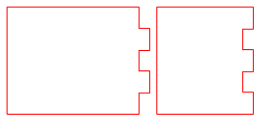
\includegraphics[width=0.5\columnwidth]{Images/fingerjoints.png}
\paragraph{How these joints look like}
Fingerjoints only consist of 90 degrees angles. Both, the female and male joints, are the same only offset by one joint. This means that the joints can slide directly into each other. But that only works when the sizes are measured correctly so that they create a tight fit. Otherwise plates connected by fingerjoints do not fit into each other at all or fall apart and have to be glued. 
\paragraph{How these joints work, and for what material}
When using fingerjoints one typically has 90 degree angles plates because it is the easiest to connect them in this angle. Other angles can be created but it is hard to know when the plates form the exact angle that is wanted unless the plates are part of a construction which gives them no other chance than to form the given angle.\\
Regarding the material fingerjoints are useless when flexible materials are connected with it. The problem is that a tight fit cannot be created as well in most cases. Also very thin material is not working well since fingerjoints hold up due to the friction of one plate to the other. The fewer material the less friction.\\
We usually use fingerjoints for acrylic and wood.

\subsubsection{JimJoint template}
    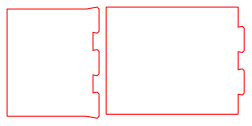
\includegraphics[width=0.5\columnwidth]{Images/jimjoints.png}
    These joints are named after Jim McCann who thankfully showed us the design for these connections.
    \paragraph{How these joints look like}
    The male and female joints are the same but they grow wider with its height. This means these joints cannot slide into each other but they rather snap together. This means once they are connected they cannot be taken apart just by pulling on the plates. 
    \paragraph{How these joints work, and for what material}
    In order for the snapping to work the material used has to be flexible or very thin and therefore flexible. Jim McCann already used it for foam. We now use it especially for paper because this material would be much too thin for creating enough friction for fingerjoints to work.

\subsubsection{Dovetail template}
    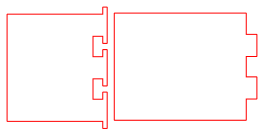
\includegraphics[width=0.5\columnwidth]{Images/schwalbe.png}
    \textbf{TODO: Image of wood dovetails where this joint is derived from.}\\
    Typically a dovetail joint is used in woodwork. It helps to ensure that when there was a pulling force on both wooden plates that the joints would all hold onto the other plate.\\
    But in order to create the female joints the wood needs to be cut in an angle. This is not possible without inadequately high time and power consumption. See the upcoming section 'alternative solution' for information on how to lasercut the female part of a dovetail.
    \paragraph{How these joints look like}
    \paragraph{How these joints work, and for what material}

\subsection{adjusting fingerjoints length when plates are angled}
    \paragraph{adjustJointHeight}
    Not only the width has to be adjusted but also the height needs to be adapted to the plates connection. Depending on the angle of the plates the joints need to be longer or shorter accordingly unless the angle is 90. With an angle of 90 the height is simply the thickness of the plates. \\
    Firstly, the angle can be projected onto values between 0 and 90. Then the cosine function returns a number between 0 and 1 for the angle. The thickness of the plate is divided by this number to achieve a height that fits the angle and the thickness of the plates. \\
    \textbf{TODO: verify the height computation and provide image}\\
    Something weird happened: I seem to have dismissed dustins calculations and try to use trigonometry. But either i cannot find the triangle i was working with or the angle in the triangle is not necissarily the angle between the plates!! Figure that out!! And make image of the trigonomety if it was correct (I remember to have done stuff on tinkercad to come to the idea maybe that helps)\\
    I really believe that I was working with a wrong angle and that this angle would be 90-alpha when alpha is smaller than 90 degrees but i dont know how to get the other angle...\\ maybe just take dustins calculations.

\section{Alternative solutions / related work}
    \begin{itemize}
        \item Snap fits we already tried. Hard to implement because enough space needs to be given when cutting the spring.
        \item how to lasercut the female part of a dovetail with alot of effort!\\
        In order to achieve different depths of cutting you can set the lasercutter to use lower power. This is usually used for engraving which also does not cut through the material.\\  
        \textbf{TODO: Name Lasercut like a boss here and include the image of the gradient which defines the power of the laser.}\\
        By coloring a part in the svg-file in a gradient from white to black this part will be cut in an angle. The more white the less power.
        \item other joint type: pettis joint (fingerjoint with screws)
        \item slot joinery technique when overlapping plates had to be rejoined
    \end{itemize}
    
    
    
\section{Future work}
    \begin{itemize}
        \item joints should not stand out on the side. \\
        Either their width has to be adjusted to be not only the width of when the joint starts building away from the plate. but also include how far away it is growing to the sides in its full height. \\
    (Beware that the joints still have to be placed according to its inner with otherwise they are too lose (except for fingerjoints) )
        \item when creating fingerjoints do not calc femaleJointsPerSide (unneccessary since using the stencilBox)
    \end{itemize}


\end{document}